\documentclass[11pt]{article}
\topmargin       -5.0mm
\headheight       0.0mm
\headsep          0.0mm
\oddsidemargin    0.0mm
\evensidemargin   0.0mm
\textheight       210mm
\textwidth        175mm

\usepackage{amsmath,amsfonts,amsthm,amssymb}
\usepackage{latexsym,mathrsfs}
\usepackage{graphicx}
\usepackage{enumerate}
\usepackage{latexsym}
\usepackage{color}
\usepackage{pstricks}
\usepackage{overpic}
\usepackage[ruled,vlined,algosection,linesnumbered]{algorithm2e}
\usepackage{subfigure}
%\usepackage{hyperref}
\usepackage{url}
\usepackage{multirow}

\newtheorem{proposition}{Proposition}[section]
\newtheorem{theorem}{Theorem}[section]
%\newtheorem{algorithm}{Algorithm}[section]
\newtheorem{lemma}{Lemma}[section]
\newtheorem{definition}{Definition}[section]
\newtheorem{corollary}{Corollary}[section]
\newtheorem{remark}{{\sc Remark}}[section]
\newtheorem{example}{Example}[section]

%\numberwithin{algorithm}{section}
\numberwithin{equation}{section}
\numberwithin{figure}{section}
\numberwithin{table}{section}

%%%%%%%%%%%%%%%%%%%%%%%%%%%%%%%%%%%%%%%%%%%%%%%%%%%%%%%%%%%%%%%%%%%%%%%%%%%%%%%%

\begin{document}

\title{On the Block Chebyshev Davidson Algorithm for PSVD}

\author{Zheng Wang}

\maketitle

%\section{Algorithm}
%\label{alg}

\section{Numerical Studies}
\label{num_study}

We test the bchdav\_svd algorithm on the matrices 'Nytimes' and 'News20' to study the effect of three important parameters: polynomial degree (\textit{polym}), block size (\textit{blk}) and maximum active subspace dimension (\textit{vimax}). In our experiment, maximum subspace dimension (\textit{vomax}) is set to a large number such that no outer restart occurs.

\subsection{Effect of the polynomial degree}

With all other parameters fixed, increasing the polynomial degree would
\begin{enumerate}
\item increase \#mat-vec-product each time the filter is used;
\item reduce \#iteration, reorthogonalization cost and refinement cost (due to larger eigenvalue gaps).
\end{enumerate}
Therefore, if we start from a small \textit{polym} and gradually increase it, total CPU time cost would probably first reduce and then increase after some large polym.\\

Table (\ref{effect_polym}) summarizes parameters used to test the effect of \textit{polym} on the convergence. Fig.(\ref{news20_polym}) -- Fig.(\ref{nytimes_polym3}) show the results of our experiments. The numerical results are consistent with our expectation except for $polym = 12$ in Fig.(\ref{nytimes_polym1}). When \textit{polym} goes from $10$ to $12$, both \#mat-vec-product and \#iteration grow rapidly. We also want to mention that in these 4 tests, bchdav\_svd does not converge when $polym$ is larger than $12$.

\begin{table}
\begin{center}
\begin{tabular}{|c|c|c|c|c|}
\hline
Matrix & k & blk & vimax & polym \\
\hline
News20 & 100 & 20 & 100 & 1:1:12\\
\hline
Nytimes & 100 & 20 & 100 & 2:2:12\\
\hline
Nytimes & 100 & 10 & 60 & 2:2:10\\
\hline
Nytimes & 100 & 5 & 40 & 2:2:10\\
\hline
\end{tabular}
\end{center}
\caption{parameters used to test the effect of polynomial degree}
\label{effect_polym}
\end{table}

\begin{figure}
\centering
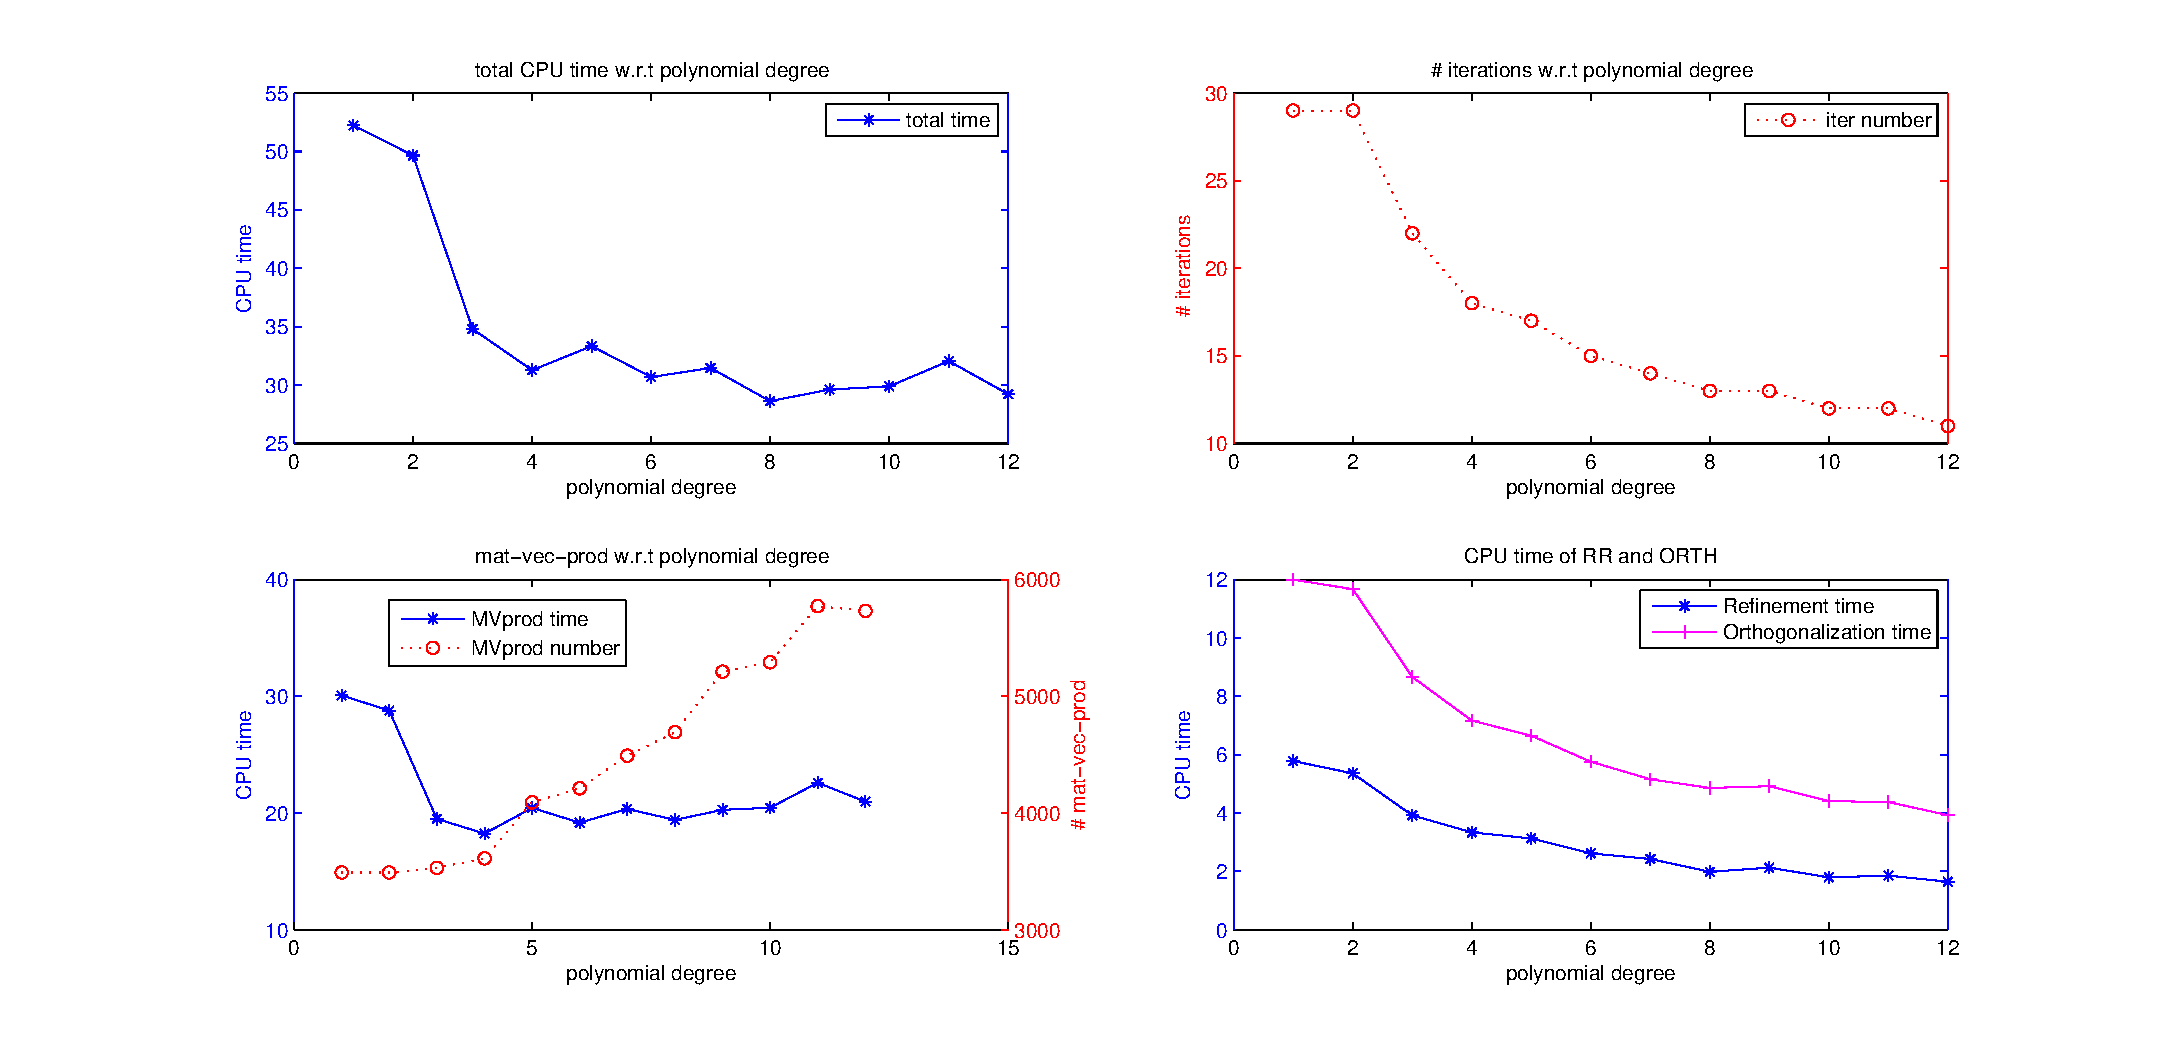
\includegraphics[scale=0.5]{news20_polym_blk20_v100.eps}
\caption{The effect of polym on converging $100$ largest singular triplets for News20 with $blk = 20$, $vimax = 100$.}
\label{news20_polym}
\end{figure}

\begin{figure}
\centering
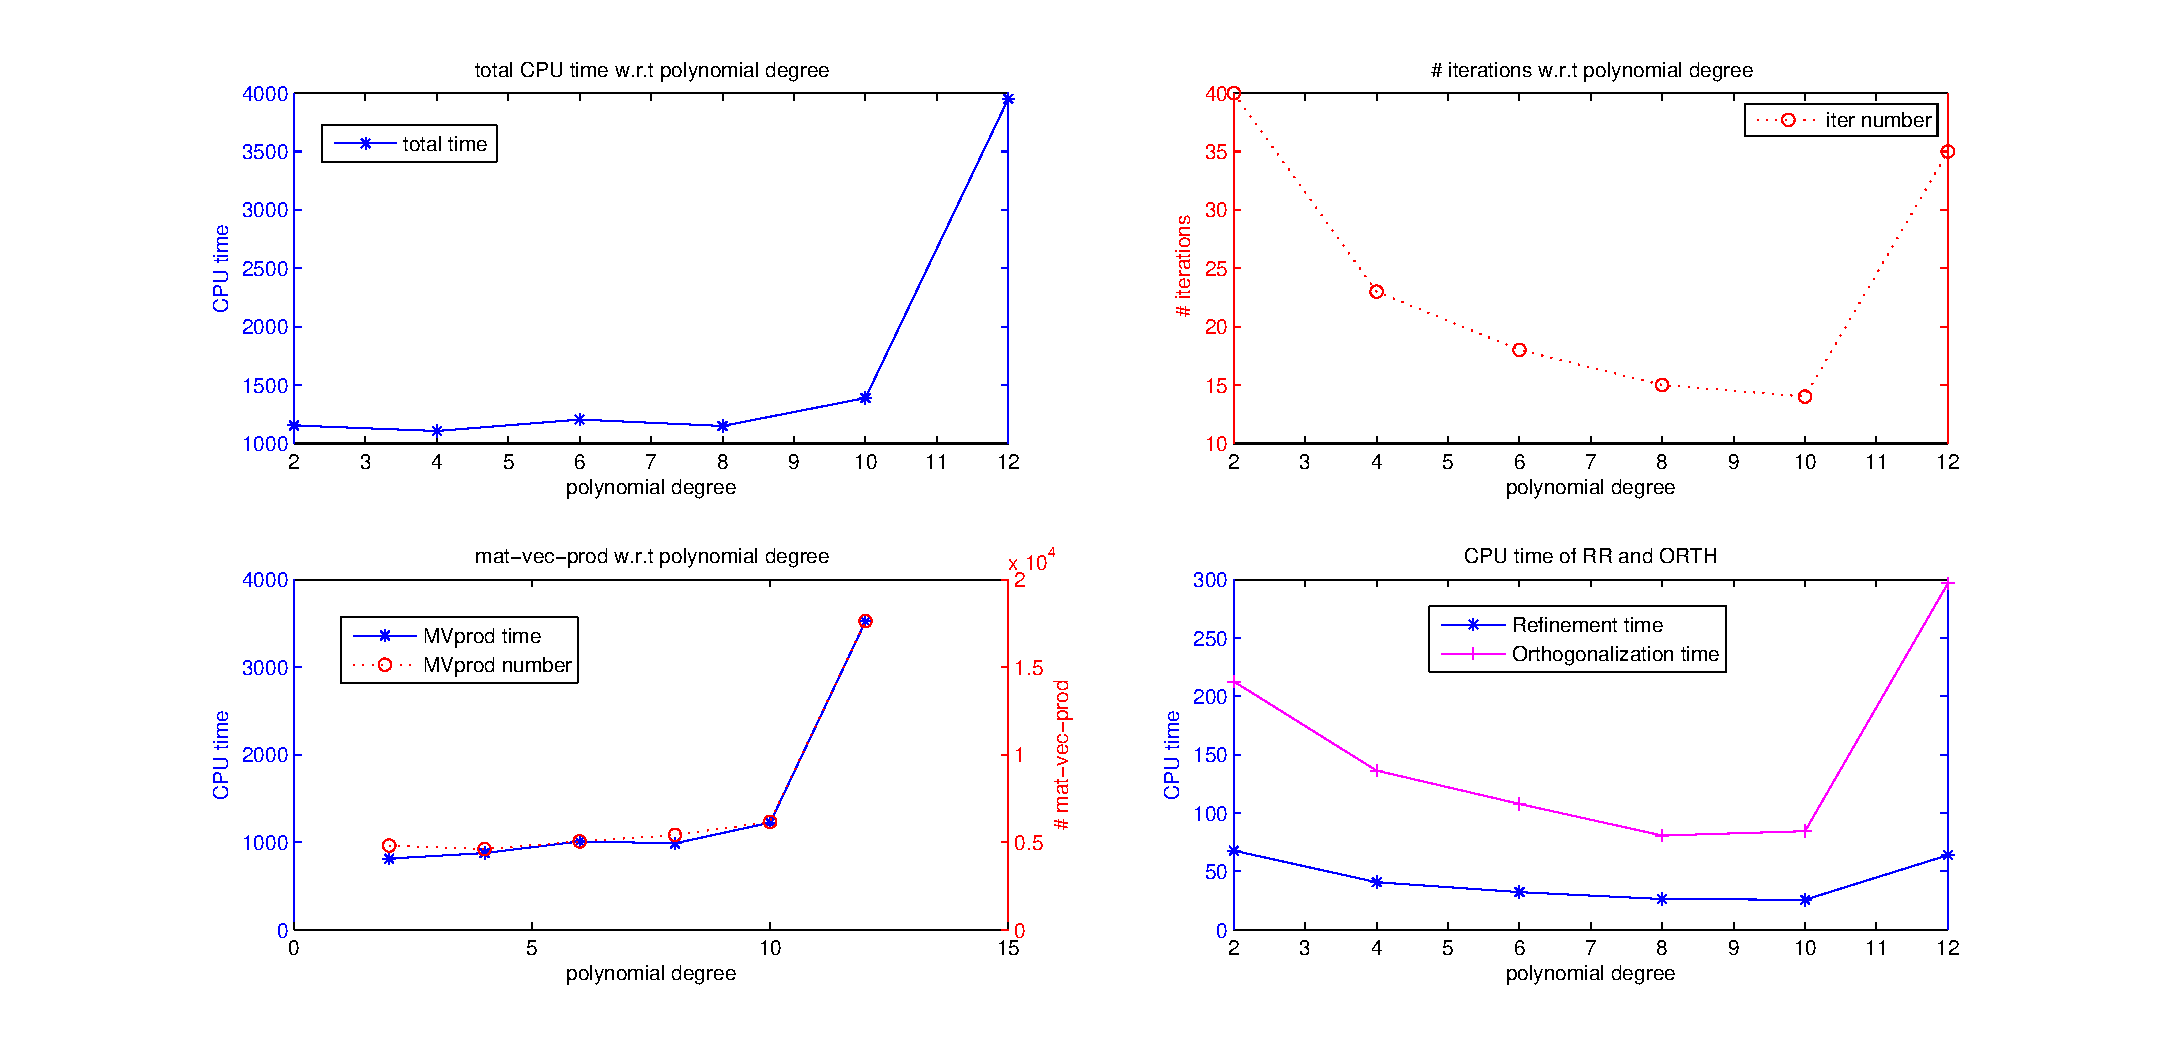
\includegraphics[scale=0.5]{nytimes_polym_blk20_v100.eps}
\caption{The effect of polym on converging $100$ largest singular triplets for Nytimes with $blk = 20$, $vimax = 100$.}
\label{nytimes_polym1}
\end{figure}

\begin{figure}
\centering
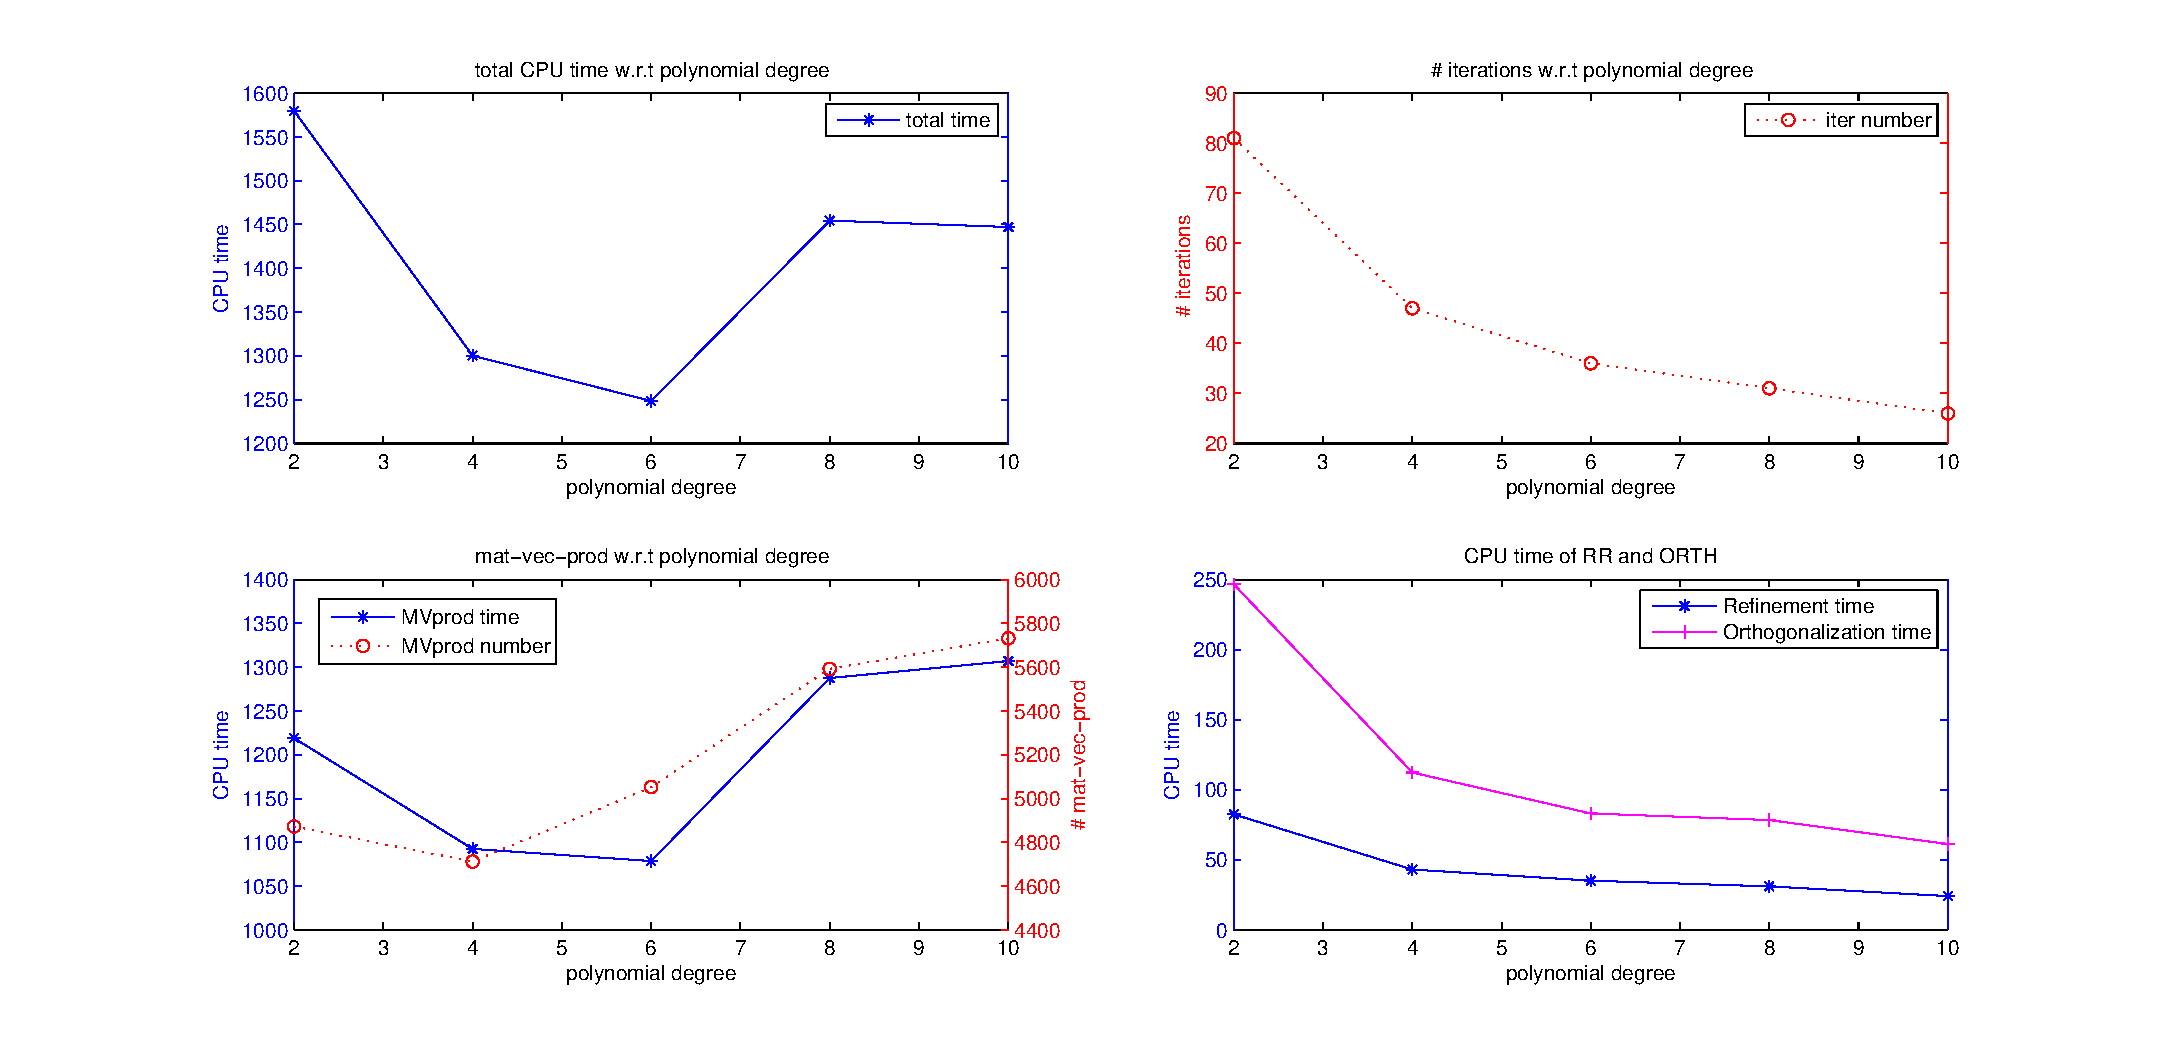
\includegraphics[scale=0.5]{nytimes_polym_blk10_v60.eps}
\caption{The effect of polym on converging $100$ largest singular triplets for News20 with $blk = 10$, $vimax = 60$.}
\label{nytimes_polym2}
\end{figure}

\begin{figure}
\centering
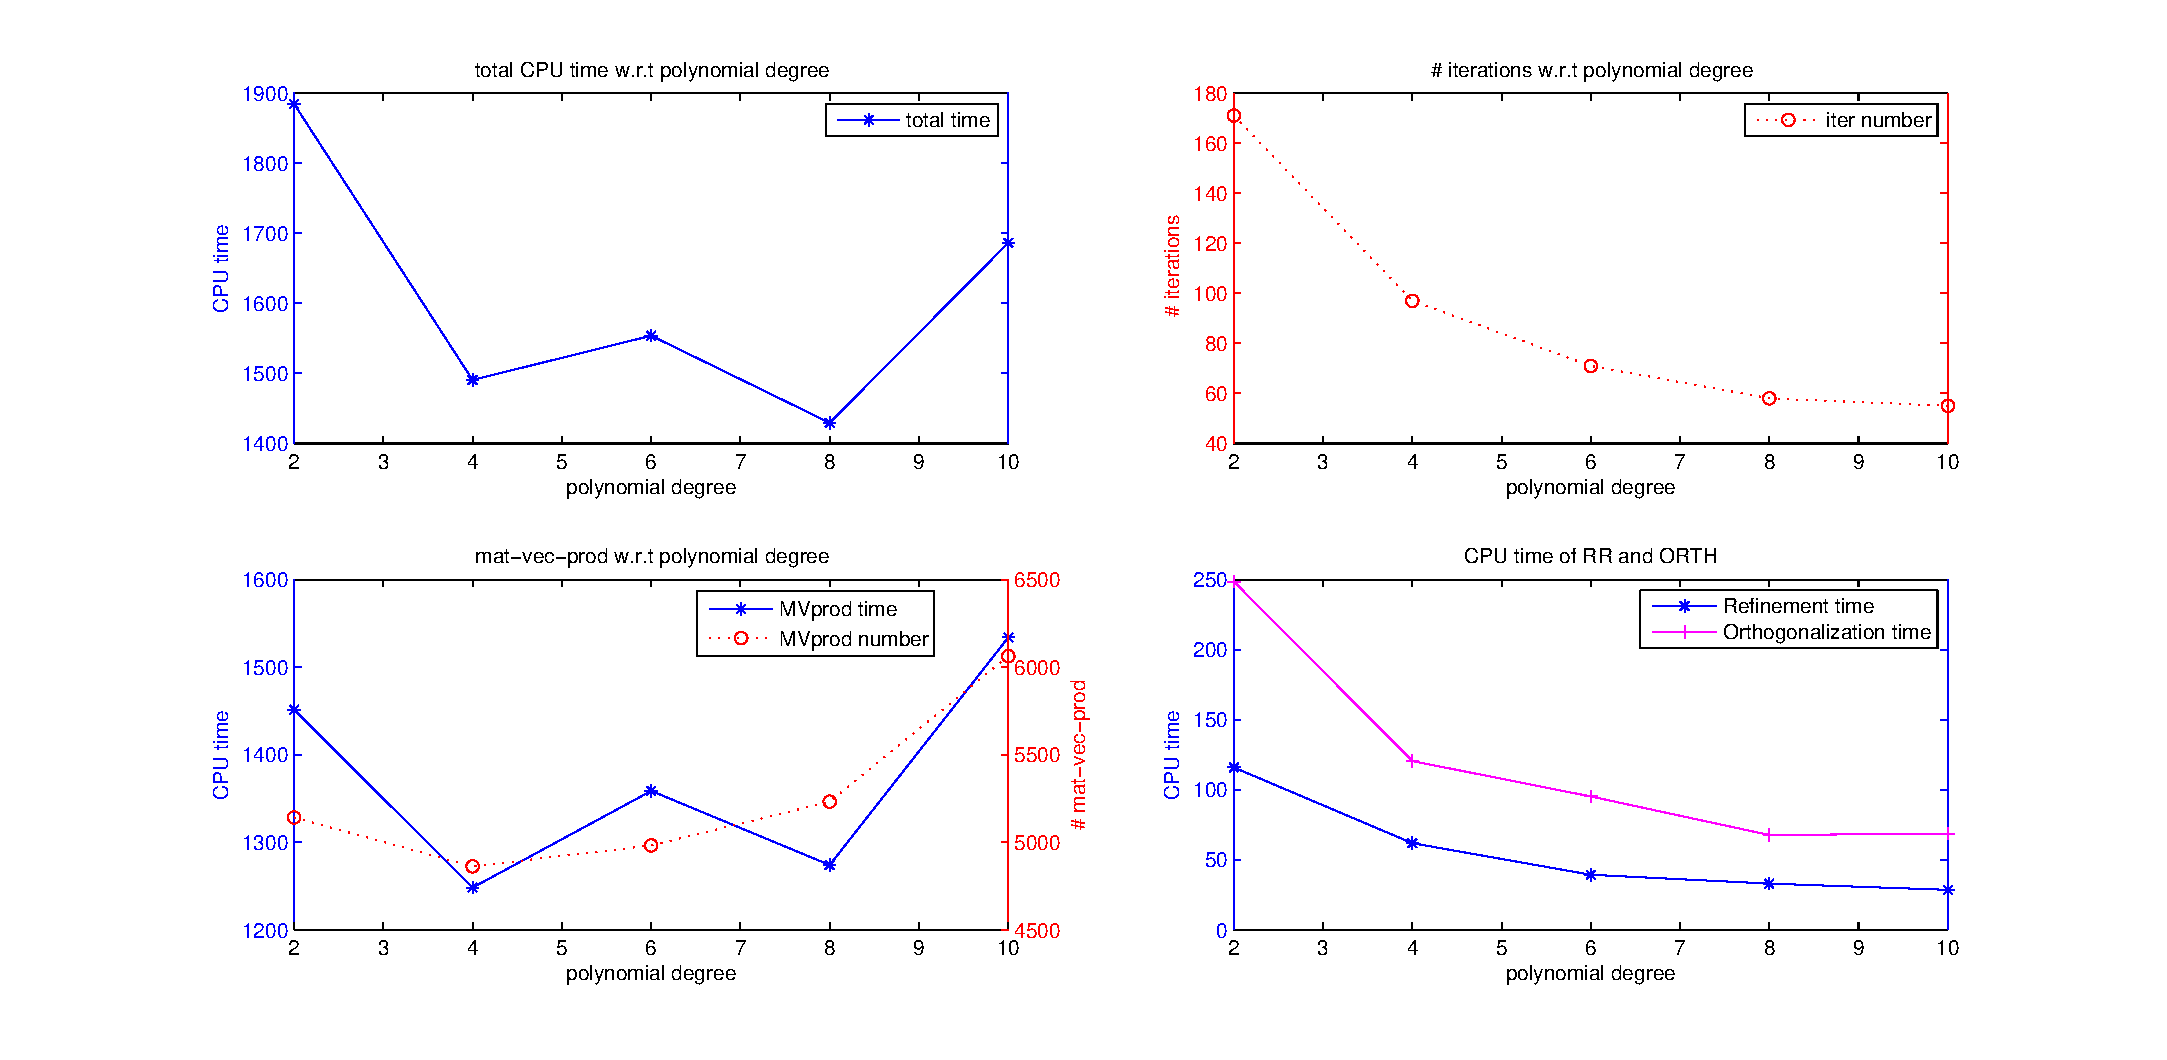
\includegraphics[scale=0.5]{nytimes_polym_blk5_v40.eps}
\caption{The effect of polym on converging $100$ largest singular triplets for News20 with $blk = 5$, $vimax = 40$.}
\label{nytimes_polym3}
\end{figure}
\subsection{Effect of the block size}


\subsection{Effect of the maximum active subspace dimension}
\bibliographystyle{plain}
\bibliography{PSVD_bib}


\end{document}
